%% RiSE Latex Template - version 0.5
%%
%% RiSE's latex template for thesis and dissertations
%% http://risetemplate.sourceforge.net
%%
%% (c) 2012 Yguaratã Cerqueira Cavalcanti (yguarata@gmail.com)
%%          Vinicius Cardoso Garcia (vinicius.garcia@gmail.com)
%%
%% This document was initially based on UFPEThesis template, from Paulo Gustavo
%% S. Fonseca.
%%
%% ACKNOWLEDGEMENTS
%%
%% We would like to thanks the RiSE's researchers community, the 
%% students from Federal University of Pernambuco, and other users that have
%% been contributing to this projects with comments and patches.
%%
%% GENERAL INSTRUCTIONS
%%
%% We strongly recommend you to compile your documents using pdflatex command.
%% It is also recommend use the texlipse plugin for Eclipse to edit your documents.
%%
%% Options for \documentclass command:
%%         * Idiom
%%           pt   - Portguese (default)
%%           en   - English
%%
%%         * Text type
%%           bsc  - B.Sc. Thesis
%%           msc  - M.Sc. Thesis (default)
%%           qual - PHD qualification (not tested yet)
%%           prop - PHD proposal (not tested yet)
%%           phd  - PHD thesis
%%
%%         * Media
%%           scr  - to eletronic version (PDF) / see the users guide
%%
%%         * Pagination
%%           oneside - unique face press
%%           twoside - two faces press
%%
%%		   * Line spacing
%%           singlespacing  - the same as using \linespread{1}
%%           onehalfspacing - the same as using \linespread{1.3}
%%           doublespacing  - the same as using \linespread{1.6}
%%
%% Reference commands. Use the following commands to make references in your
%% text:
%%          \figref  -- for Figure reference
%%          \tabref  -- for Table reference
%%          \eqnref  -- for equation reference
%%          \chapref -- for chapter reference
%%          \secref  -- for section reference
%%          \appref  -- for appendix reference
%%          \axiref  -- for axiom reference
%%          \conjref -- for conjecture reference
%%          \defref  -- for definition reference
%%          \lemref  -- for lemma reference
%%          \theoref -- for theorem reference
%%          \corref  -- for corollary reference
%%          \propref -- for proprosition reference
%%          \pgref   -- for page reference
%%
%%          Example: See \chapref{chap:introduction}. It will produce 
%%                   'See Chapter 1', in case of English language.

\documentclass[en,twoside,onehalfspacing,bsc]{risethesis}

\usepackage{natbib}
\usepackage{babel}
\usepackage{supertabular}
\usepackage{microtype}
\usepackage{lscape}
 


%% Change the following pdf author attribute name to your name.
\usepackage[linkcolor=blue,citecolor=blue,urlcolor=blue,colorlinks,pdfpagelabels,pdftitle={Karla
Malta's Bachelor Thesis},pdfauthor={Karla Malta}]{hyperref}

\address{SALVADOR}

\universitypt{Universidade Federal da Bahia}
\universityen{Federal University of Bahia}

\departmentpt{Depertamento de Ci\^{e}ncia da Computa\c{c}\~{a}o}
\departmenten{Computer Science Department}

\programpt{Programa Multiinstitucional de P\'{o}s-gradua\c{c}\~{a}o em Ci\^{e}ncia da Computa\c{c}\~{a}o}
\programen{Bachelor's Degree in Computer Science}

\majorfieldpt{Ci\^{e}ncia da Computa\c{c}\~{a}o}
\majorfielden{Computer Science}

\title{SPLICE-FeDRE: a SPL Domain Requirements Specification Tool}
\date{November/2015}

\author{Karla Malta Amorim da Silva}
\adviser{Eduardo Santana de Almeida}
\coadviser{Raphael Pereira de Oliveira}

\begin{document}

\frontmatter
\frontpage
\presentationpage

\begin{dedicatory}
I dedicate this dissertation to my family, friends and
professors who gave me all necessary support to get here.
\end{dedicatory}

%%\acknowledgements
%%Agradeço a Deus por ter me dado oportunidade de realizar este trabalho,
% saúde
%%e energia para superar todas as dificuldades. Também por cada uma das pessoas
%%citadas abaixo, que de alguma forma contribuíram para que essa conquista
% fosse possível.

%%Agradeço aos meus pais, José Carlos e Suely, por tudo que me ensinaram, por
%%acreditarem em mim e por todo suporte e incentivo para a minha formação
%%pessoal e profissional. À minha irmã, Karoline, pela sinceridade e amizade.
% Ao meu namorado, Heitor, pela cumplicidade, carinho e companhia.

%%Agradeço ao meu orientador, Dr. Eduardo Almeida, por investir em mim e guiar
% o meu trabalho. Agradeço também ao meu co-orientador, Dr. Raphael Oliveira, pela
%%disponibilidade e por compartilhar seus conhecimentos e experiências de vida.

%%Agradeço a todos os docentes do Departamento de Ciência da Computação com
%%quem tive a oportunidade de aprender durante os anos do curso de Ciência da
%%Computação, especialmente à Dra. Aline Andrade, pelos seus conselhos e
%%orientação. Agradeço ao Dr. Luciano Oliveira, pela excelência do seu
%%trabalho como professor e  coordenador do curso.  Agradeço também ao Dr.
% John McGregor por me receber no seu grupo de pesquisa e orientar durante o meu
%%estágio de verão na Universidade de Clemson (USA), onde fiz minha
% graduação sanduíche.

%%Agradeço aos meu amigos que influenciaram positivamente e participaram direta
% ou indiretamente da minha formação: Nanci Bonfim, Melissa Wen, Laiza
% Camurugy,
%%Gabriel Uaquim, Rodrigo Vieira, Félix Farias, Caio Almeida e Diego Arize.
%%Agradeço também à minha amiga Marie Cudd por me adotar em Clemson e marcar
%%minha vida de uma forma extraordinária.

%%Agradeço à Universidade Federal da Bahia por me proporcionar esta
% formação, à Fapesb, pela bolsa de Iniciação a Extensão, à Capes pela bolsa do
%%programa Ciência sem Fronteiras, e às instituições onde estagiei,
% EcGlobalPanel, IFBA, TecnoTrends e Ericsson Inovação. 


\begin{epigraph}[]{Proverbs 3:13}
Blessed is the man who finds wisdom, the man who gains understanding. 
\end{epigraph}

\resumo
% Escreva seu resumo no arquivo resumo.tex

A engenharia de software é uma disciplina que integra processos, métodos e ferramentas para o desenvolvimento de programas de computador. Para apoiá-la existem sistemas de gerenciamento de ciclo de vida de aplicativos (ALM), que são ferramentas de software que auxiliam na organização e moderação de um projeto ao longo de seu ciclo de vida. Existe um número infinito de possibilidades para definir o ciclo de vida de um projeto, e as ferramentas necessárias para ajudá-la a conclusão. Consequentemente, uma enorme variedade de sistemas de gestão estão disponíveis no mercado, especificamente concebidos de acordo com um número diversificado de metodologias de gestão. No entanto, a maioria dos sistemas são proprietários, bastante especializados e com pouca ou nenhuma capacidade de personalização, tornando muito difícil encontrar um que se encaixam perfeitamente às necessidades do seu projeto.

Um tipo diferente de desenvolvimento de sistemas de software é a Engenharia de Linha de Produtos de Software - ELPS. LPS é uma metodologia para o desenvolvimento de uma diversidade de produtos de software relacionados e sistemas com uso intensivo de software. Durante o desenvolvimento de uma LPS, uma vasta gama de artefatos devem ser criados e mantidos para preservar a consistência do modelo de família durante o desenvolvimento, o e que é importante para controlar a variabilidade SPL e a rastreabilidade entre os artefatos. No entanto, esta é uma tarefa difícil, devido à heterogeneidade dos artefatos desenvolvidos durante engenharia de linha de produto. Manter a rastreabilidade e artefatos atualizados manualmente é um processo passível de erro, demorado e complexo. Utilizar uma ferramenta para apoiar essas atividades é essencial.

Neste trabalho, propomos o Ambiente Construção Integrado de Linha de Produto de Software (SPLICE). Essa é uma ferramenta online de gerenciamento de ciclo de vida que gerencia, de forma automatizada, as atividades da linha de produtos de software. Esta iniciativa pretende apoiar a maior parte das atividades do processo de LPS, como escopo, requisitos, arquitetura, testes, controle de versão, evolução, gestão e práticas ágeis. 

Nós apresentamos um metamodelo leve, que integra o processo de ciclo de vida das Linhas de Produtos com práticas ágeis, a implementação de uma ferramenta que utiliza o metamodelo proposto , e um estudo de caso que reflete a viabilidade e flexibilidade desta solução especialmente para diferentes cenários e processos.


\begin{keywords}
ferramenta, busca
linha de produtos de software, métodos ágeis, LPS , sistema de gerenciamento de ciclo de vida de aplicativos  , ferramenta, metamodelo

\end{keywords}

\abstract
% Write your abstract in a file called abstract.tex


Software engineering is a discipline that integrates process, methods, and tools for the development of computer software. To support it, Application lifecycle management systems are software tools that assist in the organization and moderation of a project throughout its life cycle. There is an infinite number of possibilities to define a project life cycle, and the needed tools to help it completion. Consequently, a huge variety of management systems are available on today's market, specifically designed to conform to a diverse number of management methodologies. Nevertheless, most are proprietary, very specialized, with little to no customization, making very hard to find one that perfectly fit one's needs.

A different type of software systems development is Software Product Line Engineering -- SPLE. SPL is a methodology for developing a diversity of related software products and software-intensive systems. During the development of a SPL, a wide range of artifacts needs to be created and maintained to preserve the consistency of the family model during development, and it is important to manage the SPL variability and the traceability among those artifacts. However, this is a hard task, due to the heterogeneity of assets developed during product line engineering. Maintaining the traceability and artifacts updated manually is error-prone, time consuming and complex. Utilizing a tool for supporting those activities is essential. 

In this work, we propose the Software Product Line Integrated Construction Environment (SPLICE). That is a web-based life cycle management tool for managing, in an automated way, the software product line activities. This initiative intends to support most of the SPL process activities such as scoping, requirements, architecture, testing, version control, evolution, management and agile practices. This was archived with the integration of a framework around an established tool, providing an easy way for handling the usage of different metamodels.

We present a lightweight metamodel which integrates the processes of the SPL lifecycle agile practices, the implementation of a tool that uses the proposed metamodel, and a case study that reflect the feasibility and flexibility of this solution especially for different scenarios and processes



\begin{keywords}
software product line, agile, SPL, Application lifecycle management , tool, metamodel
\end{keywords}

% Summary (tables of contents)
\tableofcontents

% List of figures
\listoffigures

% List of tables
\listoftables

% List of acronyms
% Acronyms manual: http://linorg.usp.br/CTAN/macros/latex/contrib/acronym/acronym.pdf
\listofacronyms
\begin{acronym}[ACRONYM] 
% Change the word ACRONYM above to change the acronym column width.
% The column width is equals to the width of the word that you put.
% Read the manual about acronym package for more examples:
%   http://linorg.usp.br/CTAN/macros/latex/contrib/acronym/acronym.pdf




  %\acro{ALM}{Application Lifecycle Management }
  %\acro{AP}{Agile Planning }
  %\acro{BTT}{Bug Report Tracker Tool}
  %\acro{C.E.S.A.R.}{Recife Center For Advanced Studies and Systems}
  \acro{CAD}{Core Asset Development}
  %\acro{CASE}{Computer-Aided Software Engineering}
  %\acro{CRUD}{Create, read, update and delete }
  \acro{FeDRE}{Feature-Driven Requirements Engineering}
  \acro{FeDRE2}[FeDRE\textsuperscript{2}]{Feature-Driven Requirements
  Engineering Evolution}
  \acro{RE}{Requirements Engineering}
  \acro{RiSE}{Reuse in Software Engineering}
  %\acro{RQ}{Requirements}
  %\acro{ORM}{Object-relational mapping}
  \acro{PD}{Product Development}
  \acro{SPL}{Software Product Line}
  \acro{SPLE}{Software Product Line Engineering}
  \acro{SE}{Software Engineering}
  %\acro{SW}{Software}
  %\acro{SC}{Scoping}
  \acro{SPLICE}{Software Product Line Integrated Construction Environment}
  %\acro{SWIG}{Simplified Wrapper and Interface Generator}
  %\acro{TE}{Tests}
  %\acro{OT}{Others}
  %\acro{VCS}{Version control systems }    
  \acro{VM}{Variability Management}
    
\end{acronym} 

% List of listings
%\lstlistoflistings

\mainmatter

\chapter{Introduction}
\label{ch:introduction} 
A \acf{SPL} is outlined as a collection of similar software intensive systems
that share a set of common features satisfying the wants of specific customers, market segments 
or mission. Those similar software systems are developed from a set of core assets, comprised of 
documents, specifications, components, and other software artifacts that may be reusable throughout 
the development of each system within the product line
\citep{rafael2013systems}.

Requirements are typical assets in \ac{SPL}. They are specified in reusable models,
in which commonalities and variabilities are documented explicitly. Thus, these 
requirements can be instantiated and adapted to derive the requirements for an 
individual product \citep{cheng2007research}. New products in the SPL will be
much simpler to specify, because the requirements are reused and tailored
\citep{clements2002software}.

\acf{RE} in \ac{SPL} has an additional cost. Many \ac{SPL} requirements are
complex, interlinked, and divided into common, variable and product-specific requirements 
\citep{birk2003report,de2014defining}.  The requirements engineering process
must be tool-supported to handle complexity and the huge volume of elicited requirements
\citep{birk2003report}.

The focus of this dissertation is to provide a support tool for performing the specification of the 
\ac{SPL} requirements in a systematic way through the use of guidelines,  showing step by step how the 
specification should be done.

This chapter contextualizes the focus of this dissertation and starts by
presenting its motivation in \secref{sc:motivation} and a clear definition of the problem in 
\secref{sc:problem}. A brief overview of the proposed solution is presented in
\secref{sc:related}, while \secref{sc:outofscope} describes some aspects that
are not directly addressed by this work.
\secref{sc:contributions} presents the main contributions,  
\secref{sc:design} presents the research design  and, finally,
\secref{sc:structure} outlines the structure of this dissertation.

\section{Motivation}
\label{sc:motivation}
Within the \ac{SPL} paradigm, it is very important to perform a good requirements
engineering phase, because it is the basis of the  \ac{SPL} paradigm. However, existing 
tools are not designed to support the requirements engineering process for software 
product lines. Existing tools support only single product development and therefore 
lack support for modeling commonalities and variabilities as well as variation points in 
requirements \citep{birk2003report}.

Some approaches have been proposed to perform the specification and evolution of
the \ac{SPL} requirements in a systematic way through the use of guidelines: 
\acf{FeDRE} and \acf{FeDRE2}.
These approaches are considered easy to use and useful, however, they do not have a support tool. 
The lack of tool support can lead to mistakes during the manual execution of the guidelines, moreover, 
without a tool support these approaches can have problems with scalability.

In this sense, a \ac{SPL} Requirements Engineering tool is proposed to automatize the
\ac{SPL} requirements specification activities according to the \ac{FeDRE} approach. This tool is 
an extension of the \ac{SPLICE} tool \citep{splice2014cbsof}, which is an
integrated tool for developing \ac{SPL}.

\section{Problem Statement}
\label{sc:problem}

This work investigates the problems of complexity and scalability in \ac{SPL}
requirements specification phase to understand its activities in order to improve 
automation of these activities. This work promotes effort and mistakes reduction during 
SPL requirements specification by poviding a \ac{SPL} Requirements Engineering tool .   

\section{Related Work}
\label{sc:related}
In order to accomplish the goal of this dissertation, we propose the \acf{SPLICE}.
This tool supports the \acf{SPL} process activities in order to assist engineers in the traceability, variability management and maintenance activity.
The remainder of this section presents the context where it was developed and the outline of the proposed solution.

\subsection{Context}
This dissertation describes a tool that is part of the \ac{RiSE} \citep{Almeida2004}, formerly
called RiSE Project, whose goal is to develop a robust framework for software
reuse in order to enable the adoption of a reuse program. RiSE Labs it is
influenced by a series of areas, such as software measurement, architecture,
quality, environments and tools, and so on, in order to achieve its goal. The
influence areas can be seen in \figref{fg:rise-spiral}.

%\usepackage{graphics} is needed for \includegraphics
\begin{figure}[htp]
\begin{center}
  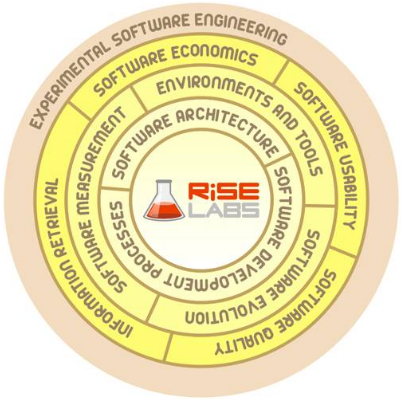
\includegraphics[width=9cm]{chapters/introduction/rise-spiral.png}
  \caption[RiSE Labs Influences]{RiSE Labs Influences}
  \label{fg:rise-spiral}
\end{center}
\end{figure}

Based on these areas, the RiSE Labs is divided in several projects, as shown in
Figure \ref{fg:rise-projects}. As it can be seen, this framework embraces
several different projects related to software reuse and software engineering.
They are:

\begin{itemize}
  \item \textbf{RiSE Framework:} Involves reuse processes
  \citep{Almeida2004,Nascimento2008}, component certification
  \citep{Alvaro2006} and reuse adoption process \citep{Garcia2008a}.
  
   \item \textbf{RiSE Tools:} Research focused on software reuse tools, such
   as the Admire Environment \citep{Mascena2006}, the Basic Asset Retrieval
   Tool (B.A.R.T) \citep{Santos2006}, which was enhanced with folksonomy
   mechanisms \citep{Vanderlei2007}, semantic layer \citep{Durao2008},
   facets \citep{Mendes2008} and data mining \citep{Martins2008}, and the
   Legacy InFormation retrieval Tool (LIFT) \citep{Brito2007}, the
   Reuse Repository System (CORE) \citep{CoreICSR}, and the Tool for Domain
   Analysis (ToolDAy) \citep{lisboa:msc:2008}. This dissertation is part of the RiSE tools;
   
   \item \textbf{RiPLE:}  Stands for RiSE Product Line Engineering Process and aims at developing   a methodology for Software Product Lines, composed of scoping \citep{Moraes2010},   requirements engineering \citep{neiva:msc:2009}, design \citep{filho:msc:2010,Cavalcanti:2011:ERP:2000259.2000286} , implementation, test \citep{neto:msc:2010,machado:msc:2010}, and evolution  management \citep{oliveira2009}.
   
   
   
   \item \textbf{SOPLE:} Development of a methodology for Service-Oriented Product Lines, based on the fundamentals of the RiPLE \citep{ribeiro2010}. 
   
   
   \item \textbf{MATRIX:} Investigates the area of measurement in reuse and
   its impact on quality and productivity;
   
   \item \textbf{BTT:} Research focused on tools for detection of duplicate
   bug reports, such as in \citet{CavalcantiFISL2008,CavalcantiInTech2012}.
   
   \item \textbf{Exploratory Research:} Investigates new research directions
   in software engineering and its impact on reuse;

   \item \textbf{CX-Ray:} Focused on understanding the \ac{C.E.S.A.R.}, and its
   processes and practices in software development.
\end{itemize}

This dissertation is part of the \ac{RiSE} Tools project. It was conducted in collaboration with researchers in software reuse , to solve the problem of traceability during the life-cycle of a\acf{SPL} development.


\begin{figure}[htp]
\begin{center}
  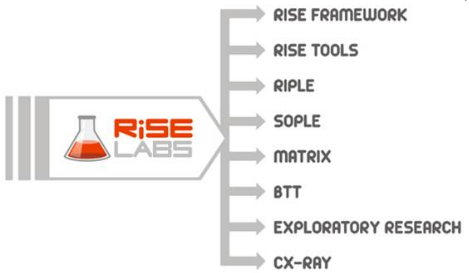
\includegraphics[width=10cm]{chapters/introduction/rise-projects.png}
  \caption[RiSE Labs Projects]{RiSE Labs Projects}
  \label{fg:rise-projects}
\end{center}
\end{figure}

\subsection{Outline of the Proposal}
This work defines the requirements, design and implementation of a software product lines lifecycle management tool, providing traceability and variability management and supporting most of the SPL process activities such as scoping, requirements, architecture, testing, version control, evolution, management and agile practices. In order to address it, we propose a metamodel that covers the SPL lifecycle, and develop a solution that consists in a Web based, extensible SPL lifecycle management tool, implementing this metamodel.  

The tool must enable the engineers involved in the process, to automatize the assets creation and maintenance, while providing traceability and variability management between them, providing detailed reports and enable the engineers to easily navigate between the assets using the traceability links. It must also provide a basic infrastructure for development, and a centralized point for user management among different tools.


\section{Out of Scope}
\label{sc:outofscope}
The following topics are not considered in the scope of this dissertation: 
\begin{itemize}
\item \textbf{SPL Domain Requirements Evolution}

Although an approach has already been proposed for the SPL domain requirements
evolution phase (FeDRE2), we still do not support this approach, but it is certainly a 
direction we intend to follow in the future.
\item \textbf{SPL Application Requirements Engineering}

In this work we do not consider the SPL Application Engineering process, then our contributions do 
not cover  the \ac{SPL} Application Requirements Engineering.
\item \textbf{Non-SPL Tools}

This work is concerned with Software Product Lines development and tools and
environments that support the \ac{SPL} approach. Non-SPL tools are out of scope.
\end{itemize}

\section{Statement of the Contributions}
\label{sc:contributions}
As a result of the work presented in this dissertation, the following contribution can be highlighted:
\begin{itemize}
\item \textbf{Tool support for a SPL domain requirements specification approach
(FeDRE)} 
We extended the \ac{SPLICE} tool, a \ac{SPL} lifecycle management tool
and automated \acf{FeDRE}, thus improving the automation of Software Product Lines (\ac{SPL}) requirements engineering phase.
\end{itemize}

\section{Research Design}
\label{sc:design}

The first step of our work was to investigate the software product line area. This informal 
study also included to understand the requirements engineering phase for single systems and 
software product lines. As a result, we could write out the second chapter with some foundations 
on these subjects.
 
During the informal study we identified the need for tools that appropriately support the domain 
requirements engineering phase of software product lines. After choosing a requirements specification 
approach (\ac{FeDRE}), we extended an existing SPL lifecycle management tool (\ac{SPLICE}) providing tool support 
for this approach.

In order to evaluate the proposed tool, we conducted a survey to identify limitations and needed 
improvements for the tool.  

\section{Dissertation Structure}
\label{sc:structure}
The remainder of this dissertation is organized as follows:

\begin{itemize}
\item \textbf{ Chapter \ref{ch:background} } reviews the essential topics
related to this work: Software Product Lines \ac{SPL}; requirements
engineering; \ac{SPL} requirements engineering; and \ac{SPLE} tool support.

\item \textbf{ Chapter \ref{ch:tool} } describes the \ac{SPLICE} tool, its
architeture and the set of frameworks and technologies used during its development. Also,  presents the new functional and non-functional 
requirements proposed for \ac{FeDRE} implementation based upon \ac{SPLICE}.

\item \textbf{ Chapter \ref{ch:survey} } describes an evaluation of \ac{FeDRE}
implementation.

\item \textbf{ Chapter \ref{ch:conclusion} } provides the concluding remarks. It
discusses our contributions, limitations, threats to validity, and outlines directions for future work.




\end{itemize}


\chapter{An Overview on Software Product Lines and CASE tools}
\label{ch:background}

\begin{quotation}[John Calt]{Dreams Come Due}
Believe nothing, no matter where you read it, or who said it, no matter if I have said it, unless it agrees with your own reason and your own common sense
\end{quotation}


\ac{SPL} has proven to be a successful approach in many business environments \citep{clements2002software}. Moreover, it is an interesting methodology for developing a diversity of software products and software-intensive systems at lower costs, in shorter time, and with higher quality \citep{Pohl2005}. Product line engineering comprises many heterogeneous activities such as capturing the variability of reusable assets, supporting the derivation of products from the product line, evolving the product line, or tailoring the approach to the specifics of a domain. The inherent complexity of product lines implicates that tool support 
is inevitable to facilitate smooth performance and to avoid costly error \citep{Dhungana2007}.CASE tools may greatly assist on maintain an efficient \acf{SPL} process, automatizing tasks, keeping traceability links and dealing with variability.

Based on the context of this work and the importance of \acf{CASE} tools on a \acf{SPL} lifecycle management, this chapter concerns the understanding of two important topics for this dissertation: Software Product Lines and \ac{CASE} tools. \secref{sc:productlines} discusses \acf{SPL}, its characteristics, development processes and benefits. 

\secref{sc:casetools} explains the \ac{CASE} Tools it applications and benefits. Recently, the term \acf{ALM} had appeared in the literature, and “has emerged to indicate the coordination of activities and the management of artifacts (e.g. requirements, source code, test cases) during the software product's lifecycle” \citep{Jukka:2009} , and we also provide a brief overview about \ac{ALM}.\secref{sc:relatedWork} addresses the what was been proposed in the literature and tools available in the market. Finally, \secref{sc:summary} presents a summary of this Chapter.



\section{Software Product Lines}
\label{sc:productlines}

\subsection{Introduction}
Nowadays, we are living in the age of customization. The customer want to have the ability to demand products that specifically address their segment or, sometimes, customer-specific adaptations to their software's \citep{rafael2013systems}.  

In today fast-paced world, companies cannot afford the luxury of not hearing what the market is asking for, and because of that, many companies have found the notion of software product lines. \acf{SPL} provide a set of work practices that allows them to drastically increase the amount of R\&D resources that focused on highly differentiating functionality and, consequently, decreasing the investment in commoditized functionality. 

A \ac{SPL} is outlined as a collection of similar software intensive systems that share a set of common features satisfying the wants of specific customers, market segments or mission. Those similar software systems are developed from a set of core assets, comprised of documents, specifications, components, and other software artifacts that may be reusable throughout the development of each system within the product line \citep{rafael2013systems}.

 \acf{SPL} is concerned with sharing common functionality within a family of products. Earlier approaches to software reuse had a tendency to focus only on the technology aspects of reusing software assets and occasionally included some process aspects. According to \citep{rafael2013systems}. Some factors that make software product lines successful is that it addresses business, architecture, process and organizational aspects of effectively sharing software assets within a portfolio of products. 


\begin{figure}[htp]
\begin{center}
  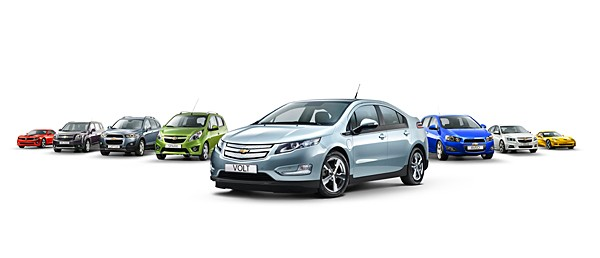
\includegraphics[width=9cm]{chapters/background/img/chev-line.jpg}
  \caption[Chevrolet Product Line]{Chevrolet Product Line.}
  \label{fg:chev-line}
\end{center}
\end{figure}


One example is General Motors , the largest automotive manufacturer in the world \citep{GmTop2012}. In 2011 it sold over nine million vehicles, produced (with its partners) in 31 countries around the world. Producing over than 1,000 vehicles off their assembly lines every hour \citep{rafael2013systems}. \figref{fg:chev-line} depicts a General Motors company and their product line of cars.


\subsection{The Benefits}

Successful introduction of a software product line provides a significant opportunity for a company to improve its competitive position \citep{rafael2013systems} , and according to \citep{ clements2002software,Pohl2005, rafael2013systems} many benefits can be identified, some examples follow:
\begin{itemize}

\item \textbf{Product portfolio diversity}

The primary and possibly most popular reason for introducing a software product line is to be able to offer a much broader and richer product portfolio against the same R\&D investment. Particularly in the case where the market is currently served by a small number of independently developed products, and can be more effectively monetized by offering more products serving smaller customer segments. More accurately, the introduction of the product line allows for effective sharing of functionality needed by all products while allowing for product-specific functionality being built on top to serve the specific market segment. \citep{rafael2013systems}.



\item \textbf{Cost reduction}

One good motive for introduce new software product line is the reduction in costs. Those reductions can come from the reuse of artifacts between a number of different systems, as is saving work to create and maintain the artifacts to each product. However, before those artifacts can be used, it should be created in a way to possibility this use, and this do not come free. This means that the company has to make an up-front investment to create the platform before it can reduce the costs per product by reusing platform artifacts.

\begin{figure}[htp]
\begin{center}
  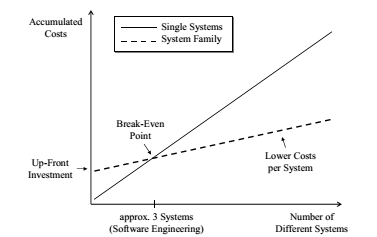
\includegraphics[width=11cm]{chapters/background/img/splcosts.png}
  \caption[Costs for developing systems as single systems compared to product 
  line engineering]{Costs for developing systems as single systems compared to product line engineering \citep{Pohl2005}}
  \label{fg:spl-costs}
\end{center}
\end{figure}

\figref{fg:spl-costs} shows the built up costs required to develop a number of different systems. The solid line sketches the costs of developing the systems independently, while the dashed line shows the costs for product line engineering. In the case of a few systems, the costs for product line engineering are relatively high, whereas they are significantly lower for larger quantities. The location at which both curves intersect marks the break-even point. At this point, the costs are the same for developing the systems separately as for developing them by product line engineering. The precise location of the break-even point depends on various characteristics of the organization and the market it has envisaged such as the customer base, the expertise, and the range and kinds of products \citep{Pohl2005}.

\item \textbf{Quality improvement}


The use of a \acf{SPL} can also bring an improvement in the overall quality of all artifacts.

A quite typical, but less publicized, alternative reason for introducing a software product line is to share one major subsystem between the products in the portfolio. One example is to share the UI framework and the generic menu structure and use cases between the products. This allows for a common look and feel across the product portfolio allowing for higher productivity of users that use different devices from the same manufacturer \citep{rafael2013systems}.

Creating the products from shared components and based on a common architecture means that the artifacts in the platform are reviewed and tested in many products. They have to prove their proper functioning in more than one kind of product. The extensive quality assurance indicates a significantly higher opportunity of detecting faults and correcting them, thereby improving the quality of all products \citep{Pohl2005}.


\begin{figure}[htp]
\begin{center}
  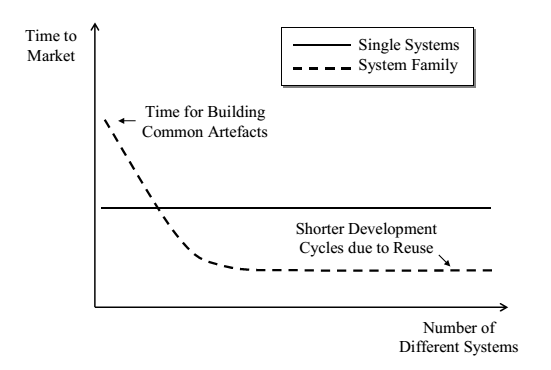
\includegraphics[width=11cm]{chapters/background/img/spl-timetomarket.png}
  \caption[Comparison of time to market with and without product line engineering]{Comparison of time to market with and without product line engineering}
  \label{fg:spl-timetomarket}
\end{center}
\end{figure}

\item \textbf{Reduction of time-to-market}


Another very important success factor for a product is the time to market.  For developing a single-product, you could do faster, in a constant time. For developing a \acf{SPL} you have an entry barrier and the time to market indeed is initially higher as the common artifacts have to be built first. However after the initial  hurdle, the time to market is considerably shortened as many artifacts can be reused for each new product, as can be seem on \figref{fg:spl-timetomarket}




\end{itemize}


\subsection{The SPL Development Process}

The \acf{SPL} Development Process has a number of definitions depending on the author. Two popular definitions on the literature \citep{clements2002software,Pohl2005} have similar interpretations that can be related to each other. \citet{clements2002software} defined three essential activities to Software Product Lines: \textbf{\acf{CAD}} activity that aims to develop assets to be further reused in other activities; \textbf{\acf{PD}} activity, which takes advantage of existing, reusable assets and \textbf{Management} activity, which includes technical and organizational management. \figref{fg:spl-activities} illustrate those activities. In addition \cite{Pohl2005} defined a framework for software product line engineering composed of two processes:

\begin{figure}[htp]
\begin{center}
  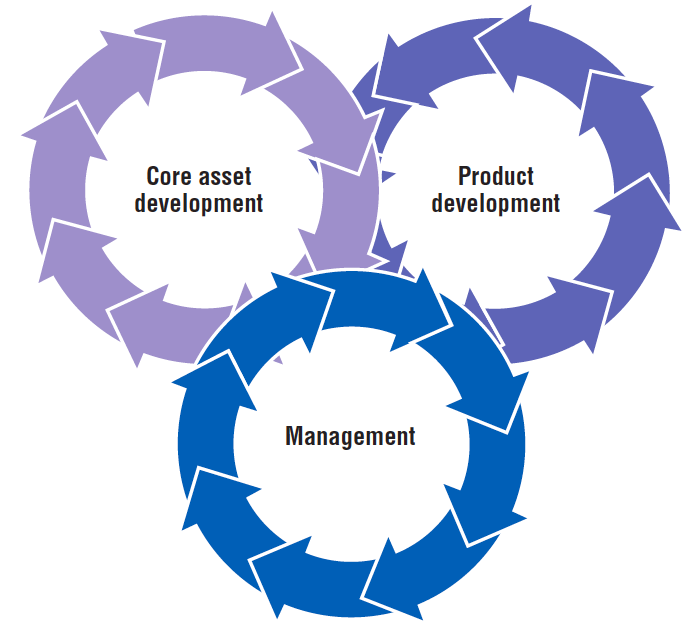
\includegraphics[width=10cm]{chapters/background/img/SPLactivities.png}
  \caption[SPL Activities]{SPL Activities \citep{clements2002software}}
  \label{fg:spl-activities}
\end{center}
\end{figure}


\begin{itemize}
\item \textbf{Domain engineering:} This process is responsible for establishing the reusable platform and thus for defining the commonality and the variability of the product line.
\item \textbf{Application engineering:} This process is responsible for deriving product line applications from the platform established in domain engineering;
\end{itemize}
An Overview of this framework can be seen in \figref{fg:spl-pohlframework}.  In essence those two approaches are related, where  \acf{CAD} activity is the Domain engineering process, and the \acf{PD} activity is the Application engineering process. Lastly, the management activity control the execution of the whole process. 





\begin{figure}[htp]
\begin{center}
  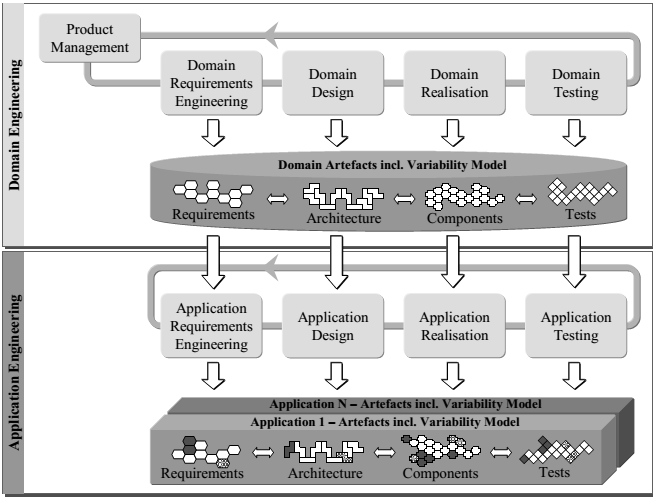
\includegraphics[width=13cm]{chapters/background/img/pohl-framework.png}
  \caption[The software product line engineering framework]{The software product line engineering framework \citep{Pohl2005}}
  \label{fg:spl-pohlframework}
\end{center}
\end{figure}





\subsubsection{Core Asset Development}


\acf{CAD}, also called by \citep{Pohl2005} as \textit{domain engineering}, it’s an activity that results in the common assets that in conjunction compose the product line’s platform \citep{clements2002software}.The key goals of this activity are \citep{Pohl2005}:
\begin{itemize}
\item Define the commonality and the variability of the software product line.
\item Specify the set of applications the software product line is planned for.
\item Determine and construct reusable artifacts that accomplish the desired variability.
\end{itemize}

In \figref{fg:spl-coreasset}, is shown the core asset development activity. This activity is interactive, and its inputs and outputs influence each other. The inputs includes product constraints; production constraints; architectural styles; design patterns; application frameworks; production strategy and preexisting assets. 
This phase is composed of the sub processes as follow \citep{Pohl2005}: 
\begin{itemize}

\item \textbf{Product Management} deals with the economic aspects associated with the software product line and in particular with the market strategy.
\item \textbf{Domain Requirements Engineering} involves all activities for eliciting and documenting the common and variable requirements of the product line.
\item \textbf{Domain Design} encompasses all activities for defining the reference architecture of the product line, 
\item \textbf{Domain Realization} deals with the detailed design and the implementation of reusable software components.
\item \textbf{Domain Testing} is responsible for the validation and verification of reusable components. 
\end{itemize}

\begin{figure}[htp]
\begin{center}
  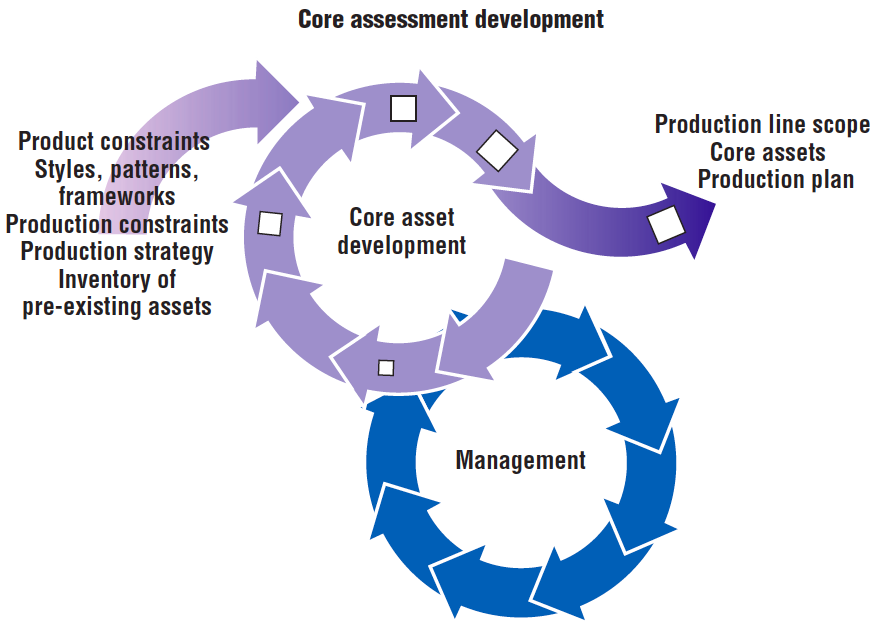
\includegraphics[width=10cm]{chapters/background/img/SPLcoreasserts.png}
  \caption[Core Asset Development]{Core Asset Development \citep{clements2002software}}
  \label{fg:spl-coreasset}
\end{center}
\end{figure}

This activity have three outputs: \textbf{Product Line Scope}, \textbf{Core Assets} and \textbf{Production Plan}. The first output, \textit{Product Line Scope}, describes the products that will constitute the product or that the product line is capable of including. Although this description can be as simple as an enumerated list, it is preferred to be detailed and carefully specified, for example, including market analysis activities in order to determine the product portfolio and to encompass which assets and products will be part of the product line. This specification must be driven by economic and business reasons to keep the product line competitive \citep{rafael2013systems}.

\textit{Core assets} are the basis for production of products in the product line. It includes an architecture that will fulfill the needs of the product line, specify the structure of the products and the set of variation points required to support the spectrum of products. It may also include components and their documentation \citep{clements2002software}.

Lastly, the \textit{production plan} describes how products are produced from the core assets. It details the overall scheme of how the individual attached processes can be fitted together to build a product \citep{clements2002software}. It is what link all the core assets together, guiding the product development within the constraints of the product line.




\subsubsection{Product Development}

\begin{figure}[htp]
\begin{center}
  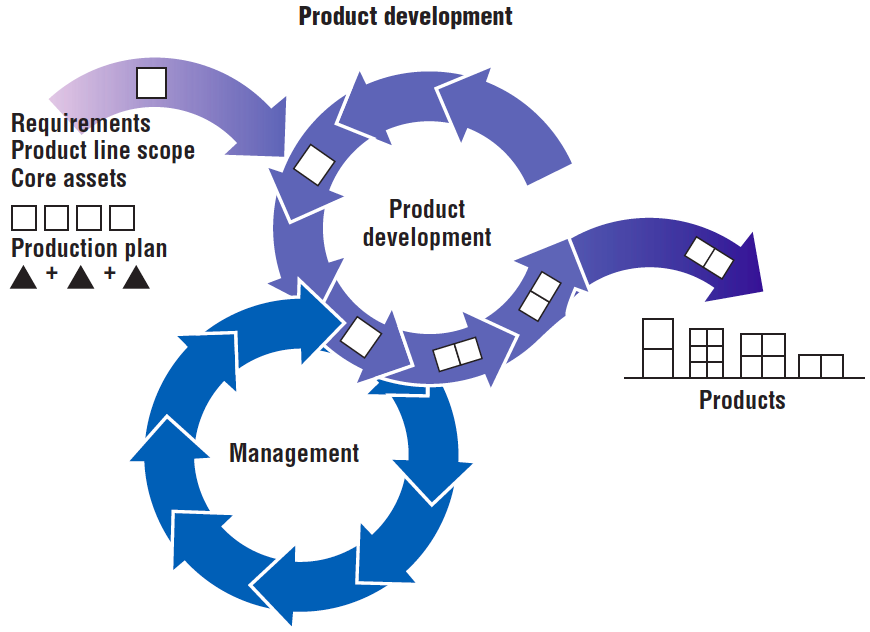
\includegraphics[width=10cm]{chapters/background/img/SPLproduct-development.png}
  \caption[Product Development]{Product Development \citep{clements2002software}}
  \label{fg:spl-productdev}
\end{center}
\end{figure}


The production plan \figref{fg:spl-productdev}, will detail how the core asserts can be used to build a product, and will be used to assemble individual product line members. The inputs for this activity are the artifacts built in the core assets development activity (product line scope, core assets, and production plan) and the requirements specification for individual products.

The outputs from this activity should be analyzed by the software engineer and the corrections must be feed back to the \acf{CAD} activity. During the product development process, some insights happens and it is important to report problems and faults encountered to keep the core asset base healthy.



\subsubsection{Management}

The management activity is responsible for the production strategy and is vital for success of the product line \citep{Pohl2005}. It is performed in two levels: technical and organizational. The technical management supervise the CAD and PD activities by certifying that both groups that build core assets and products are focused on the activities they supposed to, and follow the process. The organizational management must ensure that the organizational units receive the right resources in sufficient amounts \citep{clements2002software}.

\section{CASE Tools}
\label{sc:casetools}
\acf{CASE} tools aim to support software engineering process activities. These tools provide process support by automating some process activities and by providing information about the software that is being developed, allowing them to develop high quality systems, easy maintained and reliable (Albizuri-Romero, 2000). Their usage is greatly growing lately, because the current sophistication in SE processes means that they are hard to accomplish without reasonable tool support \citep{Dhungana2007}.

\subsection{Benefits of CASE tools}

\begin{itemize}
\item Improved communications: The communications seems to be enhanced both between project engineers and customer and among engineers working on a project;
 \item Improved documentation: The documentation improvement relates to a greater consistency and accuracy in specifying the system and in the direct generation of portions of the documentation by the CASE tools.
\item Facilitate update and modification of diagrams: The lack of tool support executing in this task makes it time consuming and difficult, and can, eventually, lead to problems in the documentation produced.
\item Assist method institutionalizing: Companies aim at achieving a more standardized way of performing software development. For that, they need a better process structure through a wider use of methods that can be easily followed. Thus, tools focused on processes (Process-Centered Software Engineering Environments -PSEE) can secure the methods rules, which can guide to an easier maintenance process.
\item Achieve a faster dialog with customers/end-users: The conversation with the customers/end-user about the product requirements, usually occur through documents and diagrams. With the tools, the manipulation of these documents/diagrams becomes faster and easier, increasing the dialogs with the customers/end-user. 

\item  Increase the work flexibility: The companies’ motivation to use CASE was the possibility of easily modifying the development methodology according to the specific situation of the product to be developed.

\item  Improve documentation: Through the improvement in documentation, companies achieve not only an easier product to maintain, but it also improves product's comprehension during customer/end-users conversations. Another motive given by the companies is that they want to improve the development reports.

\item  Reduce working effort: The tools can be useful for saving working time in routine work products, leaving more time to focus in improving the product's quality.

\end{itemize}


\subsection{Application Lifecycle Management}

The development of software products is an extremely complex undertaking, consisting of numerous interdependent activities, various different roles and a wide range of artifacts spanning over all phases of the development project and across the whole product's lifecycle \citep{lacheiner2011}. 

In the past few years, the concept of \acf{ALM} has emerged with the objective to provide a comprehensive technical solution for monitoring, controlling and managing software development over the whole application lifecycle. \citep{Schwaber2006} defines \ac{ALM} as:

“The coordination of development lifecycle activities, including requirements, modeling, development, build and testing, through: 1) enforcement of processes that span these activities; 2) management of relationships between development artifacts used or produced by these activities; and 3) reporting on progress of the development effort as a whole.” Consequently tool vendors emphasize the move towards integrated tool suites \citep{lacheiner2011}.

The \ac{ALM} as a concept is quite new and there are many conflicting definitions on what constitutes \ac{ALM}, making the whole concept of ALM is unclear and driven by tool vendors. However, \citep{kaariainen2011towards} provides a framework for \ac{ALM} that outlines what a solid process must look like.


\begin{figure}[htp]
\begin{center}
  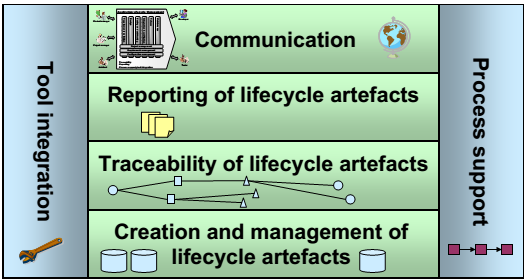
\includegraphics[width=10cm]{chapters/background/img/alm-framework.png}
  \caption[ALM Framework]{ALM Framework \citep{kaariainen2011towards}}
  \label{fg:alm-framework}
\end{center}
\end{figure}

\cite{kaariainen2011towards} came with the \ac{ALM} Framework presented on \figref{fg:alm-framework}. The elements in the middle form the levels of the \ac{ALM} elements (hierarchy) with the upper element using artifacts provided by the lower level elements. The role of process support and tool integration at the side provide an efficient working environment by equipping the elements presented in the middle to support an overall lifecycle process and tool integration. A brief description of each block, follows, \citep{kaariainen2011towards}:

\begin{itemize}

\item  \textbf{Creation and management of lifecycle artifacts} is the foundation of ALM. The product information collected and managed by this element is important for many reasons such as traceability and reporting activities.
\item  \textbf{Traceability of lifecycle artifacts} provides a means to identify and maintain relationships between lifecycle artifact, facilitating reporting, enabling change impact analysis and information visibility through the development lifecycle. 
\item  \textbf{Reporting of lifecycle artifacts} utilizes managed lifecycle artifacts and traceability information to generate needed reports from the lifecycle product information to support SW development and management. 
 \item  \textbf{Communication} enables communication tools (e.g., chat) as well as channels for distributing information on product lifecycle artifacts, links and reports and thus facilitates product information visibility for the whole \ac{SW} project. 
\item  \textbf{Process support and Tool integration} are the elements used to configure the \ac{ALM} solution to support \ac{SW} development procedures and facilitate a productive development environment by allowing the user to launch tools and transfer information easily between different tools and databases.

\end{itemize}

The \acf{SPLICE} tool developed in this work, can be considered not just a \ac{CASE} tool but, with reservations, a \acf{ALM} tool.

There are reports of \acf{ALM} tools been used to manage the Product Line engineering with  efficiency improvement, shorter lead time, and better quality in product development


\section{Tools Comparison}
\label{sc:relatedWork}

We conducted an informal search for similar commercial or academic tools. The search methodology consisted on searches on Google \footnote{http://www.google.com}, SourceForge \footnote{http://www.sf.net}, GitHub \footnote{http://www.github.com} and digital libraries of the most famous publishers and organizations in software engineering, ACM Digital Library and IEEE Computer Society Digital Library for the terms: 

\textit{“Project management”}, \textit{“Project management tool”}, \textit{“SPL project management”} and \textit{“Application Lifecycle Management”}. 

We also asked some of experts of the RiSE group, about tools they knew or heard about that would suit the task, and used the list of nineteen SPL tools compiled from the \cite{lisboa:msc:2008} thesis.

Initially we came up with \textbf{221} possible tools, and filtered using the include criteria that the tool must at least cover two areas of the \ac{SPL} process, like Requirements, Planning, Configuration management, Testing or Scoping. After the analysis, \textbf{twenty-three} tools were selected.

After the tool selection, we elected fourteen characteristics and functionalities that is interesting to be covered in an Application lifecycle tool. Table \ref{table:functionalitiestools} details which functionalities each tool offers support. The roman numbers refer to the functionalities that are described next. This table facilitates the identification of the gaps in the selected tools, and in addition it can help discovering which tool best satisfies a company’s needs.


\noindent\textbf{i) Commercial Tool}: represents if the tool is freely available, or a license is need.
\\
\\
\textbf{ii) Requirements}: provides support to include the requirements and/or use cases in the tool.
\\
\\
\textbf{iii) Agile Planning}: identifies if the tool provide support for planning using agile methodologies. 
\\
\\
\textbf{iv) Version Control Integration}: analyses if it provide integration and support for any \acf{VCS}.
\\
\\
\textbf{v) Issue Tracking}: verifies if the tool can manage issue reports. 
\\
\\
\textbf{vi) Testing}: identifies if the tool have support for activities or assets related the testing.
\\
\\
\textbf{vii) Scoping}: determines if the tool have the \textit{Feature} asset or something similar.
\\
\\
\textbf{viii) Traceability}: relates to the tool ability to provide traceability among the managed assets. 
\\
\\
\textbf{ix) Metamodel Customization}: analyses the possibility of changing and modeling the tool metamodel to specific needs. 
\\
\\
\textbf{x) Collaborative Documentation}: verifies if the tool have support for collaborative documentation such as \textit{Wikis}.
\\
\\
\textbf{xi) Web-based}: identifies if the tool have an interface that can be accessed online, or is a Desktop only product. 
\\
\\
\textbf{xii) Reports generation}: analyses if the tool can provide any kind of reports for the assets that it manages.
\\
\\
\textbf{xiii) Open-source}: specifies if the tool have the source-code publicly available.
\\
\\
\textbf{xiv) SPL oriented}: identifies if the tool is prepared or have features oriented specifically to the \ac{SPL} process.

\newcommand*\rot{\rotatebox{90}}

\begin{landscape}
\begin{table}[!ht]
\centering
\small
\tabcolsep=0.11cm
\begin{center}
    \begin{tabular}{|l|l|l|l|l|l|l|l|l|l|l|l|l|l|l|}

    \textbf{Functionalities / Tools}                         & \rot{Commercial Tool} & \rot{Requirements} & \rot{Agile Planning} & \rot{Version Control Integration} & \rot{Issue Tracking} & \rot{Testing} & \rot{Scoping}  & \rot{Traceability} & \rot{Metamodel Customization} & \rot{Collaborative Documentation} & \rot{Web-based} & \rot{Reports generation} & \rot{Open-source} & \rot{SPL oriented} \\ \hline
    BigLever  Gears           & Yes             & Yes          & No             & No                          & No             & No      & Yes            & Yes          & Partially               & No                          & No        & Yes                & No          & Yes          \\ \hline
    IBM Jazz                  & Yes             & Yes          & Yes            & Yes                         & Yes            & Yes     & Yes            & Yes          & Yes                     & No                          & Yes       & Yes                & No          & No           \\ \hline
    Polarion ALM              & Yes             & Yes          & Yes            & No                          & Yes            & Yes     & No SPL support & Yes          & Yes                     & Yes                         & Yes       & Yes                & No          & No           \\ \hline
    codeBeamer  ALM           & Yes             & Yes          & Yes            & Yes                         & Yes            & Yes     & No SPL support & Partially    & No                      & Yes                         & Yes       & Yes                & No          & No           \\ \hline
    Endeavour Agile ALM       & No              & Yes          & Yes            & Yes                         & Yes            & Yes     & No SPL support & Partially    & No                      & Yes                         & Yes       & Yes                & Yes         & No           \\ \hline
    FogBugz                   & Yes             & No           & Yes            & Yes                         & Yes            & No      & No             & No           & No                      & Yes                         & Yes       & Yes                & No          & No           \\ \hline
    FusionForge               & No              & No           & No             & Yes                         & Yes            & Yes     & No             & No           & No                      & Yes                         & Yes       & No                 & Yes         & No           \\ \hline
    Gemini Tracker            & Yes             & No           & Yes            & Yes                         & Yes            & No      & No             & No           & No                      & No                          & Yes       & Yes                & No          & No           \\ \hline
    Parasoft Concerto         & Yes             & Yes          & Yes            & No                          & Yes            & Yes     & No             & Yes          & No                      & No                          & Unknown   & Yes                & No          & No           \\ \hline
    Visual Studio TFS         & Yes             & No           & Yes            & Proprietary                 & Yes            & Yes     & No             & No           & No                      & No                          & No        & Yes                & No          & No           \\ \hline
    Workspace.com             & Yes             & Yes          & No             & No                          & Yes            & Yes     & No             & No           & No                      & Yes                         & Yes       & No                 & No          & No           \\ \hline
    Rally ALM                 & Yes             & Yes          & Yes            & No                          & Yes            & Yes     & No             & No           & No                      & Yes                         & Yes       & Yes                & No          & No           \\ \hline
    Redmine                   & No              & No           & Plugin         & Yes                         & Yes            & No      & No             & No           & No                      & Yes                         & Yes       & Yes                & Yes         & No           \\ \hline
    Trac                      & No              & No           & Plugin         & Yes                         & Yes            & No      & No             & No           & No                      & Yes                         & Yes       & Yes                & Yes         & No           \\ \hline
    Apache Bloodhound         & No              & No           & Yes            & Yes                         & Yes            & No      & No             & No           & No                      & Yes                         & Yes       & Yes                & Yes         & No           \\ \hline
    Assembla                  & Yes             & No           & Yes            & Yes                         & Yes            & No      & No             & No           & No                      & Yes                         & Yes       & Yes                & No          & No           \\ \hline
    Bontq                     & Yes             & No           & No             & No                          & Yes            & No      & No             & No           & No                      & No                          & Yes       & Yes                & No          & No           \\ \hline
    Codendi ALM               & Yes             & Yes          & Yes            & Yes                         & Yes            & Yes     & No SPL support & Yes          & No                      & Yes                         & Yes       & Yes                & No          & No           \\ \hline
    OpenProject               & No              & No           & Yes            & No                          & Yes            & No      & No             & No           & No                      & Yes                         & Yes       & Yes                & Yes         & No           \\ \hline
    Plandora                  & No              & No           & Yes            & Yes                         & Yes            & No      & No             & No           & No                      & No                          & Yes       & Yes                & Yes         & No           \\ \hline
    microTOOL in-Step         & Yes             & Yes          & Yes            & Yes                         & Yes            & Yes     & No SPL support & Yes          & No                      & No                          & No        & Yes                & No          & No           \\ \hline
    Atlassian Jira            & Yes             & No           & Yes            & Yes                         & Yes            & Plugin  & No             & No           & No                      & No                          & Yes       & Yes                & No          & No           \\ \hline
    pure::variants Enterprise & Yes             & Yes          & No             & Yes                         & No             & Yes     & Yes            & Yes          & No                      & No                          & No        & Yes                & No          & Yes          \\ \hline
    FeatureIDE & No             & Yes          & No             & Yes                         & No             & Yes     & Yes            & Yes          & No                      & No                          & No        & Yes                & No          & Yes          \\ \hline
    \end{tabular}
        \caption{Functionalities each tool supports}
        \label{table:functionalitiestools}
        \end{center}
\end{table}
\end{landscape}

\section{Summary}
\label{sc:summary}
In this chapter, we discussed about important concepts to this work: the area of \acf{SPL}, \acf{CASE} tools and \acf{ALM} tools, including motivations, benefits and definitions. We also made a analysis of features and comparison of tools available in market.

Next chapter presents the \acf{SPLICE}, a web-based, collaborative support for the \ac{SPL} lifecycle steps. It will be discussed the requirements, architecture, implementation and other aspects.


\chapter{SPLICE-FeDRE: a SPL Domain Requirements Specification Tool}
\label{ch:splice}

\section{Introduction}

In this chapter, we present functional and non-functional requirements for a tool we call SPLICE-FeDRE, 
and its implementation. The tool is an extension of \acf{SPLICE}, built in order
to support and integrate \ac{SPL} activities, such as, requirements management,
architecture, coding, testing, tracking, and release management, providing process automation and 
traceability across the process.

The remainder of this chapter is organized as follows: \secref{sc:fedre}
presents the \ac{FeDRE} approach; \secref{sc:splice} describes the tool
\ac{SPLICE}; \secref{sc:requirements} presents the requirements of SPLICE-FeDRE;
details of the implementation of SPLICE-FeDRE are discussed in
\secref{sc:implementation}; \secref{sc:operation} shows the tool SPLICE-FeDRE
in operation; and, finally, \secref{sc:solutionsummary} presents the summary of
the chapter.
 
\section{FeDRE Overview}
\label{sc:fedre}

The \acf{FeDRE} approach \citep{de2014defining} for 
\ac{SPL} has been defined by considering the feature model as the main artifact for specifying \ac{SPL} requirements. 
The aim of the approach is to perform the requirements specification by systematically utilizing the features 
identified in the \ac{SPL} domain through the use of guidelines that establish traceability links between features 
and requirements.

The main activities of the \ac{FeDRE} approach are: Scoping and Requirements Specification for Domain Engineering. 
\figref{fg:fedre-activities} shows the activities of \ac{FeDRE}, which are
detailed in this chapter. The following roles are involved in these activities: Domain Analyst, Domain Expert, Market Expert and the Domain Requirements Analyst.

\begin{figure}[htp]
\begin{center}
  \includegraphics[width=11cm]{chapters/proposed_solution/img/captures/fedre_activities.png}
  \caption[Overview of the FeDRE approach]{Overview of the FeDRE approach \citep{de2014defining}}
  \label{fg:fedre-activities}
\end{center}
\end{figure}

\subsection{Scoping}

The first activity performed in \ac{FeDRE} is the Scoping. This determines not only
what products to include in an \ac{SPL} but also whether or not an organization should 
launch the \ac{SPL}. Three main artifacts are produced as a result of the Scoping activity: 
the Feature Model, the Feature Specification, and the Product Map, using the Existing 
Assets (if any) as the input artifact. These three artifacts will drive the \ac{SPL} requirements 
specification for domain engineering. Each of these artifacts (input and outputs) is 
detailed below.

\subsubsection{Existing Assets}

Existing assets (e.g., user manual or existing systems) help the Domain Analyst
and the Domain Expert to identify the features and products in the \ac{SPL}. When they do not 
exist, a proactive approach can be followed to build the \ac{SPL} from scratch.

\subsubsection{Feature Model}

Feature modeling is a technique that is used to model common and variable
properties, and can be used to capture, organize and visualize features in the \ac{SPL}.

\subsubsection{Feature Specification}

The Domain Analyst is responsible for specifying the features using a feature
specification template. This template captures the detailed information of the
features and maintains traceability with all the artifacts involved.

\subsubsection{Product Map}

Each of the identified features is assigned to the corresponding products in the \ac{SPL}. 
The set of relationships among features and products produces the Product Map artifact, 
which describes all the features that are required to build a specific product in the \ac{SPL}.
All these artifacts are the input for the Requirements Specification for Domain Engineering 
activity, which is described next.

\subsection{Requirements Specification for Domain Engineering}

This activity specifies the \ac{SPL} requirements for domain engineering. These requirements 
allow realization of the features and desired products identified in the Scoping activity. 
The steps required to perform this activity are described in the Guidelines for Specifying 
SPL Functional Requirements, Sub-section \ref{subsec:guidelines} below.

This activity, seen in \figref{fg:fedre-activities}, uses the Feature Model,
Feature Specification and Product Map as input artifacts and produces the Glossary, Functional Requirements and Traceability Matrix 
as output artifacts. Each of these output artifacts is detailed below.

\subsubsection{Glossary}

The Glossary describes and explains the main terms in the domain in order to
provide the stakeholders with a common vocabulary and avoid misconceptions.

\subsubsection{Functional Requirements}

This artifact contains all the functional requirements identified (common or
variable), for the family of products that constitute the \ac{SPL}. Use cases are used 
to specify the \ac{SPL} functional requirements. Each functional requirement has a unique 
Use case id, a Name, a Description, Associated Feature(s), Pre and Post-Conditions, and 
the Main Success Scenario. A functional requirement can also be related to an Actor and 
may have Include and/or Extend relationships with other use case(s).

\subsubsection{Traceability Matrix}

The Traceability Matrix is a matrix that contains the links among features and
the functional requirements.

\subsection{Guidelines for Specifying SPL Functional Requirements}
\label{subsec:guidelines}

The purpose of the guidelines is to guide the Requirements Analyst in 
the specification of \ac{SPL} functional requirements for domain engineering. The 
guidelines have been structured to specify functional requirements by addressing the following 
questions: i) Which features or set of features will be grouped to be specified by use 
cases? ii) What are the specific use cases for the feature or set of features? iii) Where 
should the use cases be specified? (when there is a set of features in a hierarchy, do we specify 
the use cases for each individual feature or only for the parent features?) and iv) How is the use 
case specified in terms of steps?

Activities, tasks and steps are used in the process of specifying requirements
for \ac{SPL}. \figref{fg:fedre-guide} shows the guidelines with the detailed
steps of each task for specifying \ac{SPL} functional requirements.

\begin{figure}[htp]
\begin{center}
  \includegraphics[width=11cm]{chapters/proposed_solution/img/captures/fedre_guide.png}
  \caption[Guidelines For Specifying SPL Functional Requirements]{Guidelines For Specifying SPL Functional Requirements \citep{de2014defining}}
  \label{fg:fedre-guide}
\end{center}
\end{figure}

\section{SPLICE Overview}
\label{sc:splice}

\acf{SPLICE} \citep{splice2014cbsof}  is an open source (GNU General Public
License), Python,  web-based software product line lifecycle management tool, providing 
traceability and variability management and supporting most of the \ac{SPL} process 
activities such as scoping, requirements, architecture, testing, version control, 
evolution, management and agile practices. This tool assists the engineers involved 
in the process, with the assets creation and maintenance, while providing traceability 
and variability management, as well offering detailed reports and enabling engineers 
to easily navigate between the assets using the traceability links.

\subsection{Metamodel}

\ac{SPLICE} proposes a lightweight metamodel, representing the interactions among \ac{SPL}
assets, developed in order to provide a way of managing traceability and variability. 
The proposed metamodel represents the reusable assets involved in a \ac{SPL} project, and 
simplified description of the models is presented next.

\begin{itemize}
\item \textbf{Scoping Module} comprises the Feature and the Product Model. Many artifacts relates 
directly with the Feature Model including Use Case, Glossary, User Story and Scope Backlog. 
A Product is composed of one or more Features.

\item \textbf{Requirements Module} involves the requirements engineering
traceability and interactions issues, considering the variability and commonality in the \ac{SPL} 
products. The main object of this \ac{SPL} phase is Use Case. The concept of User stories is used 
in this metamodel to represent what a user does or needs to do as part of his or her job function. 
 
\item \textbf{Testing Module} is composed of a name, description, the
Expected result and a set of Test Steps. One Test Case can have many Test Execution that 
represent one execution of it. The reasoning for the Test Execution is to enable a test 
automation machinery. The metamodel also represents the acceptance testing with the Acceptance 
Test and Acceptance Test Execution. 

\item \textbf{Agile Planning Module} contains Sprint Planning models, which are composed of a number of Tickets, a
deadline, an objective and a start date. At the end of the sprint, it happens a retrospective, 
represented in the model by Sprint Retrospective, that contains a set of Strong Points and Should be 
Improved models that express what points in the spring was adequate, and what needs improvement.
\end{itemize}

\subsection{Main Functionalities}

The main functionalities of \ac{SPLICE} include:

\begin{itemize}
\item  \textbf{Metamodel Implementation.} All the screens are completely
auto-generated based on the models descriptions, allowing the Software Engineer to 
easily modify the process. For every model, a complete \acf{CRUD} system is
created. The \ac{SPLICE} also provides advanced features such as filtering and classification.
\item  \textbf{Issue Tracking.} \ac{SPLICE} has a full-featured Issue Tracking. It
was extended to implement \ac{SPL} specific features and to provide traceability between other assets.
\item  \textbf{Traceability.} \ac{SPLICE} provides total traceability for all assets
in the metamodel, and is able to report direct and indirect relations between them. In reports, assets 
have hyperlinks, enabling the navigation between them.
\item  \textbf{Custom SPL Widgets.} \ac{SPLICE} has a set of custom widgets to
represent specific \ac{SPL} models. Such as Feature Map, Product Map, and Agile Poker planning.
\item  \textbf{Change history and Timeline.} \ac{SPLICE} has a rich set of features
to visualize how the project is going, where the changes are happening, and who did it. For every 
Issue or Asset, a complete Change history is recorded.
\item  \textbf{Unified Control Panel.} The tool aggregates the configuration of
all external tools in a unified interface. With the same credentials, the user is able to access all 
\ac{SPLICE} features, including external tools as \acf{VCS}.
\item  \textbf{Agile Planning.} The \ac{SPLICE} supports a set of Agile practices
such as effort estimation, where team members use effort and degree of difficulty to estimate 
their own work. The Features can be dragged by the mouse, and their position is updated in accordance.
\item  \textbf{Automatic reports generation.} \ac{SPLICE} has the ability of creating
reports, including PDFs. The generated report includes a cover, a summary and the set of 
the chosen artifact related to the product. This format is suitable for the requirements 
validation by stakeholders. The tool is also able to collect all reports for a given Product, and 
create a compressed file containing the set of generated reports.
\end{itemize}

\section{SPLICE-FeDRE Requirements}
\label{sc:requirements}
In the SPLICE-FeDRE specification, the following functional requirements were
defined:

\begin{itemize}
\item  \textbf{FR1 - FeDRE Feature Specification.} The tool should provide a complete 
\ac{CRUD} (Create, Read, Update and Delete) for the model Feature that satisfies the \ac{FeDRE} 
approach needs. The model Feature should include a unique Feature id, name, description, 
priority (high, medium or low), type (abstract or concrete), variability (mandatory, optional, OR ou XOR), 
binding time (compile, runtime),  parent feature, glossary, use case diagram, similar feature(s), 
required feature(s) and excluded feature(s).

\item  \textbf{FR2 - FeDRE Use Case Specification.} The tool should provide a
complete \ac{CRUD} (Create, Read, Update and Delete) for the model Use Case that satisfies the 
\ac{FeDRE} approach needs. The model Use Case should include a unique Use case id,  name,  description, 
associated feature(s), pre-conditions, post-conditions, and the main success scenario. A Use Case can 
also be related to an actor and may have include and/or extend relationships with other use case(s), 
and alternative scenarios.

\item  \textbf{FR3 - FeDRE Guidelines.} The tool shoul implement the \ac{FeDRE}
guidelines for specifying \ac{SPL} functional requirements.  The Features must be stored  
hierarchically in order to enable \ac{FeDRE} guidelines implementation. This  should be done by 
storing Features as an n-ary tree data structure that  represents the Feature Model. 

\end{itemize}

\section{SPLICE-FeDRE Implementation}
\label{sc:implementation}

The tool \ac{SPLICE} was implemented using the Django Framework and the Python programming language. 
According to \citep{python2014}, “Python is a dynamic object-oriented
programming language that is used in a wide variety of application domains. It has a very clear, readable syntax, 
offers strong support for integration with other languages and tools, comes with extensive standard 
libraries, and can be learned in a few days. Many Python programmers report substantial productivity 
gains and feel the language encourages the development of higher quality, more maintainable code”. 
Other languages used to developed the tool were JavaScript, CSS, HTML, XML, YAML and make.

According to the \ac{SPLICE} developer, this choice was motivated by the unprecedented flexibility that 
the Django \acf{ORM} empowers it users, making the metamodel changes
effortless.
Also, Python is becoming the introductory language for a number of computer science curriculums  
\citep{Sanders2008}. Python is also frequently used on many scientific workflows
\citep{Bui2010} making the project attractive for future data scientists
experiments and for undergraduate projects.
 
The implementation of the new version called SPLICE-FeDRE adopted the same set of programming languages and 
framework for development. In SPLICE-FeDRE, the features are stored hierarchically using a modified preorder 
tree traversal algorithm. We can think of the feature model as 
an n-ary tree of features, where the root node is a special node that represents de product line. This 
tree is traversed using a depth-first search algorithm, then the \ac{FeDRE} flow of activities, tasks and 
steps is executed for each subtree of the root node, one at a time. 

\section{SPLICE-FeDRE in action}
\label{sc:operation}

In order to demonstrate how the tool SPLICE-FeDRE works, this section shows the 
operation of selected features, with a brief description.

\subsection{Feature Specification}

In the home page of SPLICE-FeDRE, seen in \figref{fg:assets}, an assets menu can
be used to manage the assets available.

\begin{figure}[htp]
\begin{center}
  \includegraphics[width=14cm]{chapters/proposed_solution/img/captures/assets.PNG}
  \caption[Assets screen]{Assets screen}
  \label{fg:assets}
\end{center}
\end{figure}

By clicking in Features, an user can have access to a complete \acf{CRUD}, 
which is also available for all the models listed in the assets menu. \figref{fg:add-feature} 
shows part of the form used to add a new Feature while specifying the Features. It implements the functional
requirement \textit{FR1- Feature Specification}. The model Feature includes a unique Feature id, 
name, description, priority (high, medium or low), type (abstract or concrete), variability 
(mandatory, optional, OR ou XOR), binding time (compile, runtime), parent feature, glossary, use case 
diagram, similar feature(s), required feature(s) and excluded feature(s). 

\begin{figure}[htp]
\begin{center}
  \includegraphics[width=14cm]{chapters/proposed_solution/img/captures/add_feature.PNG}
  \caption[Add feature form]{Add feature form}
  \label{fg:add-feature}
\end{center}
\end{figure}

\subsection{FeDRE Guidelines}

The \ac{FeDRE} page is depicted in \figref{fg:start-fedre}. Once the features
specification is finished, the user can start the flow of \ac{FeDRE} guidelines in order to specify the requirements of each subtree of features, 
one by one. It implements the functional requirement \textit{RF3 – FeDRE
Guidelines}.

\begin{figure}[htp]
\begin{center}
  \includegraphics[width=14cm]{chapters/proposed_solution/img/captures/start_fedre.PNG}
  \caption[FeDRE initial screen]{FeDRE initial screen}
  \label{fg:start-fedre}
\end{center}
\end{figure}

For each branch, the user can see a hierarchy of this branch features, and lists of the features that 
must have use cases, the features that may have use cases and the features that should not have use cases. 
Also, it is shown a list of steps to be accomplished before moving to the next
branch, as seen in \figref{fg:branch1}.

\begin{figure}[htp]
\begin{center}
  \includegraphics[width=14cm]{chapters/proposed_solution/img/captures/branch1.PNG}
  \caption[Branch example]{Branch example}
  \label{fg:branch1}
\end{center}
\end{figure}

\subsection{Use Case Specification}

As mentioned above, a complete \ac{CRUD} is also accessible for the model Use
Case.
Implementing the requirement \textit{FR2 - Use Case Specification}, the model
Use Case includes a unique Use case id,  name,  description, associated feature(s), pre-conditions, 
post-conditions, 
and the main success scenario. A Use Case can also be related to an actor and may have include and/or 
extend relationships with other use case(s), and alternative scenarios. See
\figref{fg:add-use-case} below:

\begin{figure}[htp]
\begin{center}
  \includegraphics[width=14cm]{chapters/proposed_solution/img/captures/add_use_case.PNG}
  \caption[Add use case form]{Add use case form}
  \label{fg:add-use-case}
\end{center}
\end{figure}

\section{Summary}
\label{sc:solutionsummary}

In this chapter, it was presented the \acf{FeDRE} approach and the \acf{SPLICE},
a web-based tool for \ac{SPL} lifecycle management, and how it was extended to 
automate the \ac{FeDRE} approach. Next chapter presents an evaluation of SPLICE-FeDRE 
performed during the development of the tool. 



\chapter{SPLICE-FeDRE Evaluation}
\label{ch:caseStudy}

\section{Introduction}
\label{sc:experimentIntroduction}

This chapter describes a survey applied to validate the tool developed for this
work. It is organized as follows: \secref{sc:definition} defines this evaluation; in \secref{sc:researchMethod} the 
data collection model is presented; \secref{sc:datacollection} describes the results and its interpretation; the 
\secref{sc:threats} analyzes the threats to validity of the evaluation; \secref{sc:leassonsLearned} and \secref{sc:expsummary} describe some 
findings and summarize the chapter.

\section{Definition}
\label{sc:definition}

\subsection{Context}
A survey was applied, after the complete implementation of SPLICE-FeDRE, in
order to validate the application developed in regard to its usefulness when it 
comes to handling complexity and scalability problems during requirements specification. 
The survey was applied at Software Engineering Laboratory, in November 2015, and we had 
two participants that were master students, all members of \acf{RiSE} Lab.
\subsection{Research Questions}

In this evaluation the main objective is to analyze the usefulness of the tool for handling 
complexity and scalability problems that may arise during requirements specification phase 
of a \acf{SPL}. In order to evaluate these aspects in our proposal, we 
defined two research questions:
\begin{itemize}
\item \textbf{Is the proposed tool useful for handling compexity during the SPL Requirements Engineering process?}

Rationale: The goal is to verify if the tool helps handling complexity during the \ac{SPL} 
Requirements Engineering process.
\item \textbf{Is the proposed tool useful for handling scalability problems during the SPL Requirements Engineering process?}

Rationale: The goal is to verify if the tool helps handling scalability problems during the \ac{SPL} 
Requirements Engineering process.

\end{itemize}

\section{Data collection}
\label{sc:researchMethod}

\subsection{Survey Design}
The data collection instrument selected in this evaluation is the Expert Survey. A survey is a 
mechanism of data gathering in which participants answers questions or statements previously 
developed and they are probably the most commonly used instrument to gather opinions from experts 
according to \citep{Kitchenham2008}.

This survey design is based on the design proposed by \citep{Kitchenham2008} and it is 
composed of a set of personal questions, closed-ended and open-ended questions related to the research 
questions. Also, to give the respondents the necessary understanding about the application, a training 
was offered to them. The remain of this section contains the overall process applied in this evaluation 
and the methodology used. 
\subsection{Developing the Survey Instrument}
The questionnaire was composed of three personal questions, five closed
questions with justification fields, and three open questions. The closed questions were 
formulated to measure and quality the data, while getting personal feedback. The open questions 
were built to collect the experts’ experiences and their impressions about the tool. The questionnaire 
can be seen in the Appendix 1.

\subsection{Analyzing the data}
In order to collect the data, the experts filled a printed questionnaire. After designing and running 
the survey, the next step was to analyze the collected data. The main analysis procedure was to check 
all responses, tabulate the data, identify the findings and classify the options.

\section{Results}
\label{sc:datacollection}
In this section the analysis of the collected data are presented, discussing the
given answer for each question.

\subsubsection{Respondents experience}
The first three questions were personal questions such as name and experience,
and their answers are summarized in Table \ref{table:expertsselected}.

\begin{table}
\begin{center}
\centering
\small
\tabcolsep=0.11cm
    \begin{tabular}{|l|l|l|l|}
    \hline
    Respondent & Occupation & RE experience & SPL experience           
    \\ \hline 1 & M.Sc student & 4 years & 3 years and 5 months
    \\ \hline 2 & M.Sc student & 6 years & 3 years 
    \\ \hline
    \end{tabular}
        \caption {Experts Selected}
        \label{table:expertsselected}
        \end{center}

\end{table}

\subsubsection {Tool usage difficulties}
Considering the questions \textbf{“Did you have any difficulty during the
execution of any activity in the tool?”} and  \textbf{“Did you have any problems
creating  use cases?”}, none of the respondents reported any difficulty to use
the tool.

\subsubsection{Tool Helpfulness}
In the question \textbf{“Do you think that the proposed tool would aid you
during a SPL Requirements Engineering process? Would you spontaneously use the
tool hereafter?”} all the respondents agreed that the tool would aid them to specify 
requirements and would keep using the tool 
from that moment on. However, one of them stated that the \ac{FeDRE} steps could
be more detailed in the tool.


Considering the question \textbf{“Do you think the proposed tool is useful to
handle the complexity of SPL Requirements Engineering process?”}, both
respondents answered yes, and one of them stated that the tool reduces the effort to specify 
requirements using \ac{FeDRE} guidelines.


All the respondents indicated in the question \textbf{“Do you think the proposed
tool is useful to handle scalability problems during a SPL Requirements
Engineering process?”} that the proposed tool is useful to handle scalability problems that may arise during  
\ac{SPL} Requirements Engineering process.

\subsubsection{Positive points}
We asked the experts the question \textbf{What are the positive points of using the tool?}, and the positive 
points of the tool according to them are:
\begin{itemize}
\item Centralized information;
\item More accuracy when choosing the use cases to be specified;;
\item Time saving.
\end{itemize}

\subsubsection{Negative points}
In Contrast with the previous question, we also asked \textbf{What are the
negative points of using the tool?}.
Only one point was mentioned, as follow:
\begin{itemize}
\item An external tool is needed to draw the use case diagrams.
\end{itemize}

\subsubsection{Suggestions}
Lastly, we asked \textbf{“Please, write down any suggestion you think might be
useful”}. One expert suggested that we implement a use case drawing feature as part of the tool 
to avoid the use of external tools. The another expert suggested a more illustrated interface.

\section{Threats to validity}
\label{sc:threats}
There are some threats to the validity of our study, which were briefly
described and discussed:
\begin{itemize}
\item \textbf{Research questions.} The research questions we defined cannot
provide complete coverage of all the features covered by the tool. We considered just some important points: complexity and 
scalability problems handling.

\item \textbf{Sample size.} The number of respondents is an important detail in
a survey. Due to the limited availability of respondents with a \ac{SPL} background, the evaluation
may contain biases.
A higher number of participants helps  generalizing the results obtained.

\item \textbf{Quality of training.} The quality of the training conducted before
applying the questionnaire may have compromised the correct understanding of the \ac{FeDRE} approach and 
the application evaluated.

\item \textbf{Translation of the answers.} All the responses were written in
portuguese and translated to english by the author. This may have changed the direction of the response.

\end{itemize}

\section{Findings}
\label{sc:leassonsLearned}

\section{Summary}
\label{sc:expsummary}

This chapter presented the definition, planning, analysis and interpretation of a survey 
to evaluate the SPLICE-FeDRE tool. The survey was applied to experts at Software Engineering Laboratory. 
The two participants were members of \ac{RiSE} Lab. After concluding the  
questionnaires, we gathered information that can be used as a guide to improve the tool, and an indicator 
about the actual status of the tool. 
The results of the experiment pointed out that the SPLICE-FeDRE addresses the 
complexity and scalability problems that may arise during \ac{SPL} requirements
engineering phase.
However, some points of improvements were raised, that we plan to fix on future versions. Next 
chapter presents the concluding remarks and future work of this dissertation.



\chapter{Conclusion}
\label{ch:conclusion}

\begin{quotation}[The End of the Beginning]{Winston Churchill }
Now this is not the end. It is not even the beginning of the end. But it is, perhaps, the end of the beginning.
\end{quotation}

\acf{SPL} has proven to be the methodology for developing a diversity of software products and software-intensive systems at lower costs, in shorter time, and with higher quality. Many reports document the significant achievements and experience gained by introducing software product lines in the software industry \citep{Pohl2005}. However, the complexity of product lines processes implicate that tool support is inevitable to facilitate smooth performance and to avoid costly errors \citep{Dhungana2007}. 

An upcoming concept is the \acf{ALM}, which deals with approaches, methodologies and tools for integrated management of all aspects of software development. Its goal is to making software development and delivery more efficient and predictable by providing a highly integrated platform for managing the various activities of the development lifecycle from inception through deployment \citep{kaariainen2011towards}. Chapter 2 summarized the basic concepts about software product lines, \ac{ALM} tools, \ac{CASE} tools and their aspects. We also presented an informal study of features available in commercial tools.

In this sense, in order to facilitate the process usage and to aid the \acf{SE} during the \ac{SPL} process, this dissertation presented, in Chapter 3, a lightweight metamodel for \ac{SPL} using agile methodologies. We also desbribed in details, the \acf{SPLICE} tool, build in order to support and integrate \ac{SPL} activities, such as, requirements management, architecture, coding, testing, tracking, and release management, providing process automation and traceability across the process. We presented the functional and non-functional requirements, its architecture, as well as theinvolved frameworks and technologies.

An evaluation of the \ac{SPLICE} tool was presented in Chapter 4, with a case study conducted inside the research laboratory. The results demonstrated that the \ac{SPLICE} address the traceability problem and was considered useful to all experts.

\section{Research Contribution}
\label{sc:reserach-contrib}
The main contributions of this research are described as follows:
\begin{itemize}
\item  \textbf{Informal review of available \ac{ALM} tools}. Through this study, was conducted an informal search for similar commercial or academic tools. Fourteen characteristics and functionalities that is interesting to be covered in an Application lifecycle tool.  A table was created comparing all the tools, that companies can use as a way to identify the best tool according to their needs.

\item  \textbf{ SPL Lightweight Metamodel}. Based on a previous metamodel, and the need for applying agile methodologies, we introduced a proposal for a lightweight metamodel that represents the interaction among asserts of a \ac{SPL} during its lifecycle.
\item  \textbf{ SPLICE tool}. To implement the metamodel proposed, it was presented a web-based tool for \ac{SPL} lifecycle management, including the set of functional and non-functional requirements, architecture, frameworks and technologies adopted during its construction.
\item  \textbf{Case Study}. After the tool development, a case study was performed to evaluate the \ac{SPLICE} tool and gather opinions and critics about the product, to guide further development.

\end{itemize}

\section{Future Work}
\label{sc:future-work}
An initial prototype was developed and evaluated in this work. However, we are aware that some enhancements and features must be implemented, as well as some defects must be fixed. Experts reported some of the enhancements and defects during our survey, and others were left out because they were out of scope of a graduation project. Thus, some important aspects are described as follows:

\begin{itemize}

\item  \textbf{ Visual metamodel editing}. One main objective of this work is to present a flexible tool, giving the possibility to adapt the implemented metamodel for specific project needs. Therefore, a visual editor must be implemented during the project setup to be more intuitive to users.

\item  \textbf{ Source code variation.} The tool actually do not support source-code variability, since the users are only able to perform assets derivation. With source-code variation support, we could archive a complete derivation process.

\item  \textbf{ Risk Management}. According to \cite{Sommerville2011}, Risk Management (RM) is important because of the inherent uncertainties that most projects face. We did not implement this model in our metamodel. As consequence, we intend to consider this feature in the next improvements. 

  
\item  \textbf{ Further evaluation}. In this work, we presented a case study. A more detailed evaluation is needed by applying the proposed case study protocol in other contexts in order to provide richer findings for the stakeholders. 
\end{itemize}



\bibliographystyle{natbib}
\addcontentsline{toc}{chapter}{\bibliographytocname}
\bibliography{references}

%Appendix
\clearpage
\addappheadtotoc
\appendix
\appendixpage
\chapter{Case Study Instruments}
\label{ap:measurement-instruments}


\def \tick{
$[$\hspace{0.3cm}$]$
}

\def \twooption#1#2{
\tick #1.  \tick #2.
}

\def \threeoption#1#2#3{
\tick #1.\newline
\tick #2.\newline
\tick #3.
}

\def \fouroption#1#2#3#4{
\tick #1.\newline
\tick #2.\newline
\tick #3.\newline
\tick #4.
}

\def \fiveoption#1#2#3#4#5{
\tick #1.\newline
\tick #2.\newline
\tick #3.\newline
\tick #4.\newline
\tick #5.
}
\def \datefield{
%date fied used in time sheets
    /\hspace{0.4cm}/
}

\def \rcolor{
%table row color
    \rowcolor[gray]{0.9}
}

\def \hcolor{
    \rowcolor[gray]{0.7}
}


\section{Form for Expert Survey}
\label{ap:sec:feedback}

\textbf{Name: }
\\
\line(1,0){380}
\\
\textbf{What is your experience with programming (in months/years) ? }
\\
\line(1,0){410}
\\
\line(1,0){410}
\\
\textbf{What is your experience with Software Product Lines ? }
\\
\line(1,0){410}
\\
\line(1,0){410}
\\
\textbf{There was any difficult during the execution of some activity in the tool ?}
\\
\twooption{Yes}{No}
\\
\textbf{In case you answered “Yes”,detail the difficulty encountered:}
\\
\line(1,0){410}
\\
\line(1,0){410}
\\
\line(1,0){410}
\\
\line(1,0){410}
\\
\textbf{How the usage of the tool altered your workflow ?  }
\\
\line(1,0){410}
\\
\line(1,0){410}
\\
\line(1,0){410}
\\
\line(1,0){410}
\\
\textbf{Did you have any problems creating assets ?}
\\
\twooption{Yes}{No}
\\
\textbf{In case you answered “Yes”,describe the problems encountered:}
\\
\line(1,0){410}
\\
\line(1,0){410}
\\
\line(1,0){410}
\\
\line(1,0){410}
\\
\textbf{Did the tool gave you enough information to identify who did a specific modification in an asset ?}
\\
\twooption{Yes}{No}
\\
\textbf{In case you answered “No”,describe what was missing:}
\\
\line(1,0){410}
\\
\line(1,0){410}
\\
\line(1,0){410}
\\
\line(1,0){410}
\\
\textbf{Do you consider that tool aided the traceability among the assets?}
\\
\twooption{Yes}{No}
\\
\textbf{Justify:}
\\
\line(1,0){410}
\\
\line(1,0){410}
\\
\line(1,0){410}
\\
\line(1,0){410}
\\
\textbf{Did you expect any traceability link not available in the tool ? If so, which one(s) ?}
\\
\line(1,0){410}
\\
\line(1,0){410}
\\
\line(1,0){410}
\\
\line(1,0){410}
\\
\textbf{What is your opinions on navigating among traceability links ?}
\\
\line(1,0){410}
\\
\line(1,0){410}
\\
\line(1,0){410}
\\
\line(1,0){410}
\\
\textbf{In your opinion, the reports generated were satisfactory ?}
\\
\twooption{Yes}{No}
\\
\textbf{If no , what was missing ?}
\\
\line(1,0){410}
\\
\line(1,0){410}
\\
\line(1,0){410}
\\
\line(1,0){410}
\\
\textbf{Do you think that the proposed tool would aid you during a SPL process ? Would you spontaneously use the tool hereafter?}
\\
\line(1,0){410}
\\
\line(1,0){410}
\\
\line(1,0){410}
\\
\line(1,0){410}
\\
\\
\textbf{What are the positive points of using the tool?}
\\
\line(1,0){410}
\\
\line(1,0){410}
\\
\line(1,0){410}
\\
\line(1,0){410}
\\
\\
\textbf{What are the negative points of using the tool?}
\\
\line(1,0){410}
\\
\line(1,0){410}
\\
\line(1,0){410}
\\
\line(1,0){410}
\\
\\
\textbf{Please, write down any suggestion you think might be useful.}
\\
\line(1,0){410}
\\
\line(1,0){410}
\\
\line(1,0){410}
\\
\line(1,0){410}
\\


\end{document}
